% tikzpic.tex
\documentclass[crop,tikz]{standalone}% 'crop' is the default for v1.0, before it was 'preview'

\usetikzlibrary{arrows,decorations.pathmorphing,decorations.pathreplacing,backgrounds,positioning,fit,matrix}
\usetikzlibrary{shapes,calc,patterns,arrows.meta}
\tikzset{
	vert/.style={circle,inner sep=1.5,fill=white,draw,minimum size=.3cm},
	edge/.style={color=black, thick},
	diredge/.style={->,>={Stealth[width=8pt,length=8pt]},color=black, thick},
	timelabel/.style={fill=white,font=\footnotesize, text centered},
	wave/.style={decorate,decoration={coil,aspect=0}},
	dirwave/.style={->, >={Stealth[width=8pt,length=8pt]},decorate,decoration={coil,aspect=0}},
	diredge2/.style={->,>={Stealth[width=8pt,length=8pt]}}
}
\begin{document}
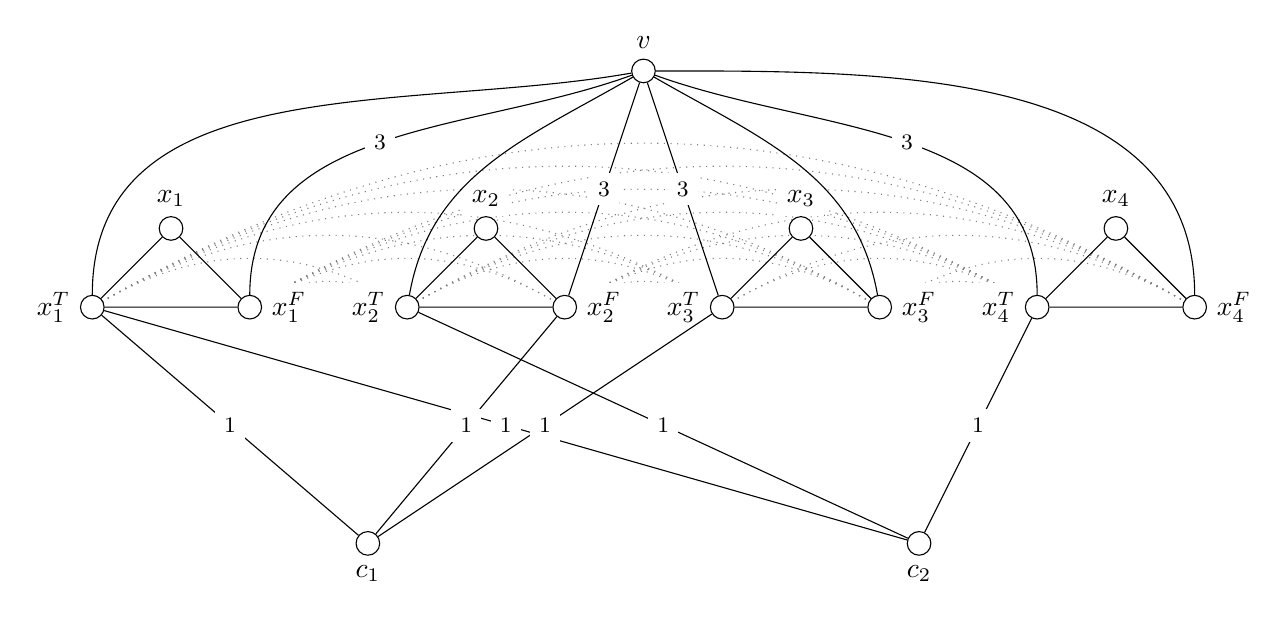
\begin{tikzpicture}%[xscale=2]
	
	%%Variable X1
	\node (x1t) at (1,0) {};
	\node (x1f) at (3,0) {};
	
	%%Variable X2
	\node (x2t) at (5,0) {};
	\node (x2f) at (7,0) {};
	
	%%Variable x3
	\node (x3t) at (9,0) {};
	\node (x3f) at (11,0) {};
	
	%%Variable x4
	\node (x4t) at (13,0) {};
	\node (x4f) at (15,0) {};
	
	%% edges among xt, xf vertices
	%x1 to all
	\draw [dotted,gray] (x1t) [out=30,in=150] to (x2t);
	\draw [dotted,gray] (x1t) [out=30,in=150] to (x3t);
	\draw [dotted,gray] (x1t) [out=30,in=150] to (x4t);
	\draw [dotted,gray] (x1t) [out=30,in=150] to (x2f);
	\draw [dotted,gray] (x1t) [out=30,in=150] to (x3f);
	\draw [dotted,gray] (x1t) [out=30,in=150] to (x4f);
	
	\draw [dotted,gray] (x1f) [out=30,in=150] to (x2t);
	\draw [dotted,gray] (x1f) [out=30,in=150] to (x3t);
	\draw [dotted,gray] (x1f) [out=30,in=150] to (x4t);
	\draw [dotted,gray] (x1f) [out=30,in=150] to (x2f);
	\draw [dotted,gray] (x1f) [out=30,in=150] to (x3f);
	\draw [dotted,gray] (x1f) [out=30,in=150] to (x4f);
	%x2 to all
	\draw [dotted,gray] (x2t) [out=30,in=150] to (x3t);
	\draw [dotted,gray] (x2t) [out=30,in=150] to (x4t);
	\draw [dotted,gray] (x2t) [out=30,in=150] to (x3f);
	\draw [dotted,gray] (x2t) [out=30,in=150] to (x4f);
	
	\draw [dotted,gray] (x2f) [out=30,in=150] to (x3t);
	\draw [dotted,gray] (x2f) [out=30,in=150] to (x4t);
	\draw [dotted,gray] (x2f) [out=30,in=150] to (x3f);
	\draw [dotted,gray] (x2f) [out=30,in=150] to (x4f);
	%x3 to all
	\draw [dotted,gray] (x3t) [out=30,in=150] to (x4t);
	\draw [dotted,gray] (x3t) [out=30,in=150] to (x4f);
	
	\draw [dotted,gray] (x3f) [out=30,in=150] to (x4t);
	\draw [dotted,gray] (x3f) [out=30,in=150] to (x4f);
	
	%%Variable X1
	\node[vert,label=left:$x_1^T$] (x1t) at (1,0) {};
	\node[vert,label={[fill=white]right:$x_1^F$}] (x1f) at (3,0) {};
	\node[vert,label=above:$x_1$] (x1) at (2,1) {};
	\draw (x1t) -- (x1f) -- (x1) -- (x1t);
	
	%%Variable X2
	\node[vert,label={[fill=white]left:$x_2^T$}] (x2t) at (5,0) {};
	\node[vert,label={[fill=white]right:$x_2^F$}] (x2f) at (7,0) {};
	\node[vert,label={[fill=white]above:$x_2$}] (x2) at (6,1) {};
	\draw (x2t) -- (x2f) -- (x2) -- (x2t);
	
	%%Variable x3
	\node[vert,label={[fill=white]left:$x_3^T$}] (x3t) at (9,0) {};
	\node[vert,label={[fill=white]right:$x_3^F$}] (x3f) at (11,0) {};
	\node[vert,label={[fill=white]above:$x_3$}] (x3) at (10,1) {};
	\draw (x3t) -- (x3f) -- (x3) -- (x3t);
	
	%%Variable x4
	\node[vert,label={[fill=white]left:$x_4^T$}] (x4t) at (13,0) {};
	\node[vert,label=right:$x_4^F$] (x4f) at (15,0) {};
	\node[vert,label=above:$x_4$] (x4) at (14,1) {};
	\draw (x4t) -- (x4f) -- (x4) -- (x4t);
	
	%%vertices for clauses c1, c2 + vertex v
	\node[vert,label=above:$v$] (v) at (8,3) {};
	\node[vert,label=below:$c_1$] (c1) at (4.5,-3) {};
	\node[vert,label=below:$c_2$] (c2) at (11.5,-3) {};
	
	%%% edges between x1 gadget and v,c1,c2
	\draw (x1t) to node[timelabel] {$1$} (c1);
	\draw (x1t) to node[timelabel] {$1$} (c2);
	\draw (x1t) to [out=90,in=190] (v);
	\draw (x1f) to [out=90,in=200] node[timelabel] {$3$} (v);
	
	%%% edges between x2 gadget and v,c1,c2
	\draw (x2f) to node[timelabel] {$1$} (c1);
	\draw (x2t) to node[timelabel] {$1$} (c2);
	\draw (x2t) to [out=80,in=210]  (v);
	\draw (x2f) to node[timelabel] {$3$} (v);
	
	%%% edges between x3 gadget and v,c1
	\draw (x3t) to node[timelabel] {$1$} (c1);
	\draw (x3t) to node[timelabel] {$3$} (v);
	\draw (x3f) to [out=100,in=330] (v);
	
	%%% edges between x4 gadget and v,c2
	\draw (x4t) to node[timelabel] {$1$} (c2);
	\draw (x4t) to [out=90,in=340] node[timelabel] {$3$} (v);
	\draw (x4f) to [out=90,in=360] (v);
	
	
\end{tikzpicture}
\end{document}